%%%%%%%%%%%%%%%%%%%%%%%%%%%%%%%%%%%%%%%%%%%%%%%%%%%%%%%%%%%%%%%%%%%%%%%
%
%   Presentation of Beamer UNL Theme
%   Beamer Presentation by Chris Bourke
%
%%%%%%%%%%%%%%%%%%%%%%%%%%%%%%%%%%%%%%%%%%%%%%%%%%%%%%%%%%%%%%%%%%%%%%%
%% Make tables with set width
\documentclass{beamer}
%% Be able to use subfigure
%\usepackage{caption}
\usepackage{subcaption}
\captionsetup{compatibility=false}

\usetheme[hideothersubsections]{UNLTheme}


\title[HAL - Protein]{HIERARCHICAL ACTIVE LEARNING (HAL) APPLICATION TO MITOCHONDRIAL DISEASE PROTEIN DATASET}
\author{James Duin} %
\institute{University of Nebraska -- Lincoln \\ Master's Thesis}
\date{Spring 2017 \\ \href{mailto:jamesdduin@gmail.com}{\color{blue}{\texttt{jamesdduin@gmail.com}}}}

\begin{document}
%{% open a Local TeX Group
%\setbeamertemplate{sidebar}{}
\begin{frame}
    \titlepage
\end{frame}
%}% end Local TeX Group










\section{Introduction}
\begin{frame}
    \frametitle{Introduction}
    \framesubtitle{}
\begin{itemize}
  \item Machine Learning
  \item Evaluating Classifier Performance
  \item Hierarchical Bioinformatics Dataset
  \item Coarse-grained vs Fine-grained Trade Off
  \item Active Over-Labeling
  \item Hierarchical Active Learning
  \item Dynamically Adapting Purchase Proportions
  \item Related Work
  \item Training and Testing Coarse-grained and Fine-grained Classifiers
  \item SVM and Logit Classifier Performance
  \item Active vs Passive Curve Analysis
  \item Plots for Fine Fixed Ratio Results
  \item BANDIT Approach Results
  \item Conclusions and Future Work
\end{itemize}
\end{frame}









\section{Background}
\begin{frame}
    \frametitle{Machine Learning}
    \framesubtitle{}
\begin{itemize}
  \item Machine learning (ML) algorithms are defined as computer programs that learn from experience E
with respect to some class of tasks T and performance measure P, if their performance at
tasks in T, as measured by P, improves with experience E - \textit{Mitchell}.
  \item Support Vector Machine
  \item Logistic Regression
\end{itemize}
\end{frame}
\begin{frame}
    \frametitle{Evaluating Classifier Performance}
    \framesubtitle{Confusion Matrix}
    \begin{itemize}
      \item True-Negatives ($T_n$): Correctly classified negative instances.
      \item False-Negatives ($F_p$): Incorrectly classified negative instances.
      \item False-Positives ($F_n$): Incorrectly classified positive instances.
      \item True-Positives ($T_p$): Correctly classified positive instances.
    \end{itemize}
    \begin{table}[H]
    \centering
    \caption{Example of a confusion matrix, with $100$ negative and $50$ positive instances in the test set.}
    \label{tab:confEx}
    \begin{tabular}{|l||l|}\hline
    conf (tn/fn) & conf (fp/tp) \\ \hline
    90 & 10 \\ \hline
    20 & 30 \\ \hline
    \end{tabular}
    \end{table}
\end{frame}
\begin{frame}
    \frametitle{Evaluating Classifier Performance}
    \framesubtitle{Precision and Recall}
    Precision is a measure of result relevancy:
    \begin{equation}
    \label{eq:precision}
    \begin{aligned}
    P = \frac{T_p}{T_p+F_p}
    \end{aligned}
    \end{equation}
    Recall is a measure of how many truly relevant results are returned:
    \begin{equation}
    \label{eq:recall}
    \begin{aligned}
    R = \frac{T_p}{T_p+F_n}
    \end{aligned}
    \end{equation}
\end{frame}
\begin{frame}
    \frametitle{Evaluating Classifier Performance}
    \framesubtitle{F-Measure}
    The F-measure or F1-measure (F1) is the harmonic mean of precision and recall:
    \begin{equation}
    \label{eq:fmes}
    \begin{aligned}
    F1 = 2\cdot \frac{P \cdot R}{P+R}
    \end{aligned}
    \end{equation}
\end{frame}
\begin{frame}
    \frametitle{Evaluating Classifier Performance}
    \framesubtitle{ROC - PR curves}
    \begin{figure}[!htb]
        \centering
        \begin{subfigure}[t]{0.5\textwidth}
            \centering
            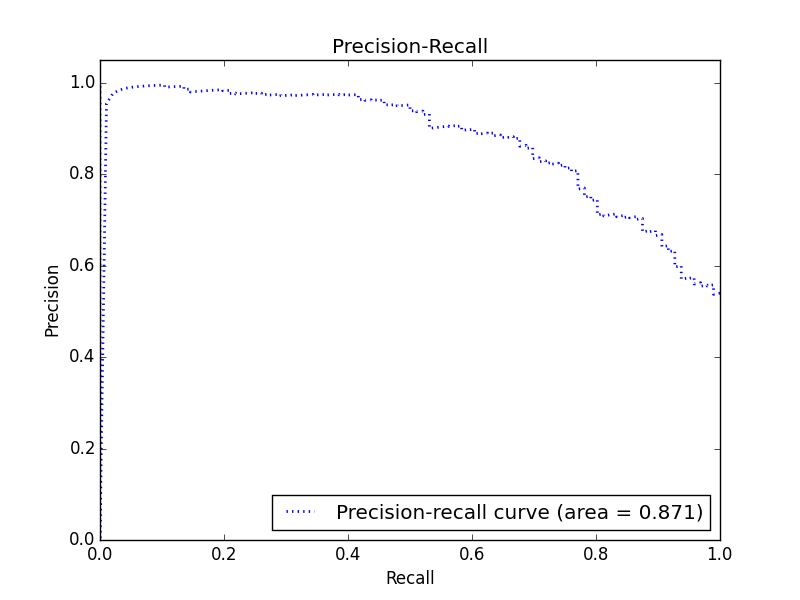
\includegraphics[width=\textwidth]{fig/Psv_1_2_fine_PR}
            \caption{PR curve.}
        \end{subfigure}%
        ~
        \begin{subfigure}[t]{0.5\textwidth}
            \centering
            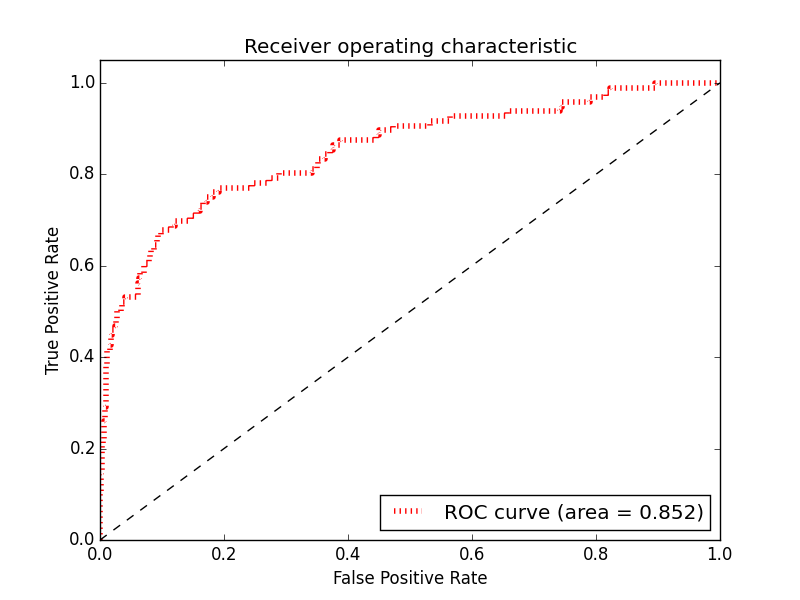
\includegraphics[width=\textwidth]{fig/Psv_1_2_fine_ROC}
            \caption{ROC curve.}
        \end{subfigure}
        \caption{Examples of PR and ROC curves with their corresponding AUC values.}
        \label{fig:PRRocExamples}
    \end{figure}
\end{frame}
\begin{frame}
    \frametitle{Hierarchical Bioinformatics Data Set}
    \framesubtitle{Feature Sources}
%    \begin{table}[H]
%      \centering
%      \small
%      \caption{Features of the protein dataset along with their respective sources.}
%      \label{tab:featureList}
%      \resizebox{1.0\columnwidth}{!}{
%      \begin{tabular}{|p{0.25\linewidth}|p{0.5\linewidth}|p{0.25\linewidth}|} \hline
%        Type of Properties & Features (dimension) & Sources \\ \hline
%        General sequence features & Amino acid composition (20), sequence length (1), etc. %di-peptides composition (400)
%        & Calculated by Kevin Chiang at UNL \\
%         & Normalized Moreau-Broto, autocorrelation (240), etc.
%%         Moran autocorrelation (240), Geary autocorrelation (240),
%%         Sequence order (160), Pseudo amino acid composition (50)
%         & PROFEAT \\ \hline% \cite{PROFEAT1} \\ \hline
%        Physico chemical properties &  Hydrophobicity (21), normalized Van der Waals volume (21), etc.
%%        polarity (21), polarizability (21), charge (21), secondary structure (21)
%%        and solvent accessibility (21)
%        & Computed
%%        with composition (C),
%%        transition (T), and distribution (D)
%        from Cui et al. \\ %\cite{Cui2} \\
%         & Solubility (1), unfold-ability (1), etc. &
%        %disorder regions (3), global charge (1) and hydrophobility (1) &
%        PROSO and Phobius \\ \hline %\cite{PROSO3}, Phobius \cite{Phobius4} \\ \hline
%        Structural properties & Secondary structural content (4), shape
%        (Radius Gyration) (1) & SSCP \cite{PSSCP5} \\ \hline
%        Domains and motifs & Signal peptide (1), transmembrane domains
%        (alpha helix and beta barrel) (5), Glycosylation
%        (both N-linked and O-linked) (4),
%        Twin-arginine signal peptides motif (TAT) (1) & SignalP \cite{SignalP6},
%        TMB-Hunt \cite{TMBHunt7}, NetOgly \cite{NetOgly8}, TatP \cite{TatP9} \\
%          \hline
%      \end{tabular} }
%    \end{table}
\end{frame}
\begin{frame}
    \frametitle{Hierarchical Bioinformatics Data Set}
    \framesubtitle{Labeling Hierarchy}
    \begin{figure}[!htb]
        \centering
    %    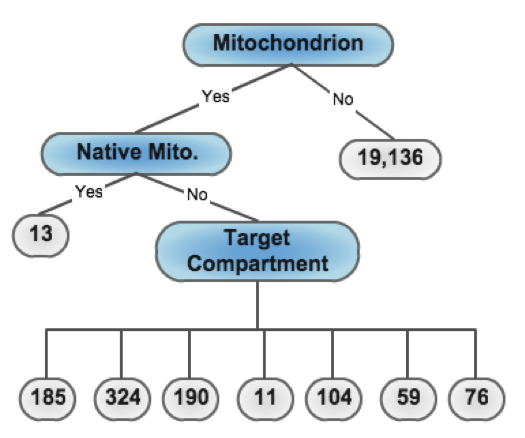
\includegraphics[width=0.75\columnwidth]{fig/Mito_tree}
    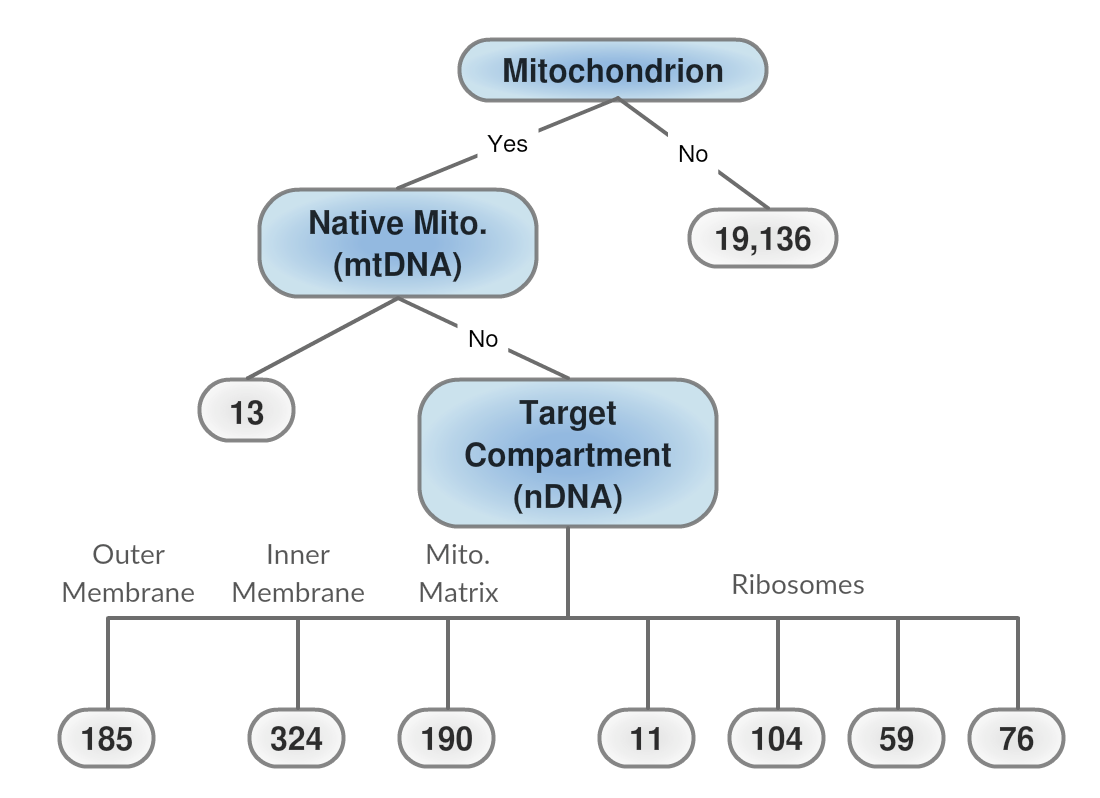
\includegraphics[width=0.75\columnwidth]{fig/MitoTreeLabels}
        \caption{The protein dataset hierarchy of labels along with the instance
        count for each label.}
        \label{fig:Mitotree}
    \end{figure}
\end{frame}
\begin{frame}
    \frametitle{Coarse-grained vs Fine-grained Trade Off}
    \framesubtitle{}
    \begin{figure}[!htb]
	\centering
    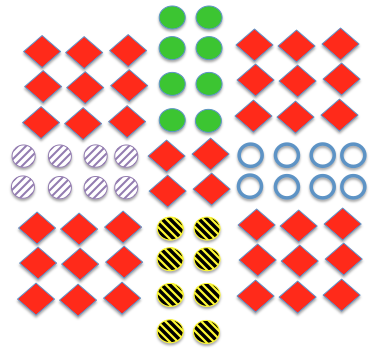
\includegraphics[width=0.5\columnwidth]{fig/union}
    \caption{Demonstration of a dataset that would benefit from multiple fine-grained
    learners for each circle type, from Mo et al.}
    \label{fig:union}
\end{figure}
\end{frame}
\begin{frame}
    \frametitle{Active Over-Labeling}
    \framesubtitle{}
    \begin{figure}[!htb]
        \centering
        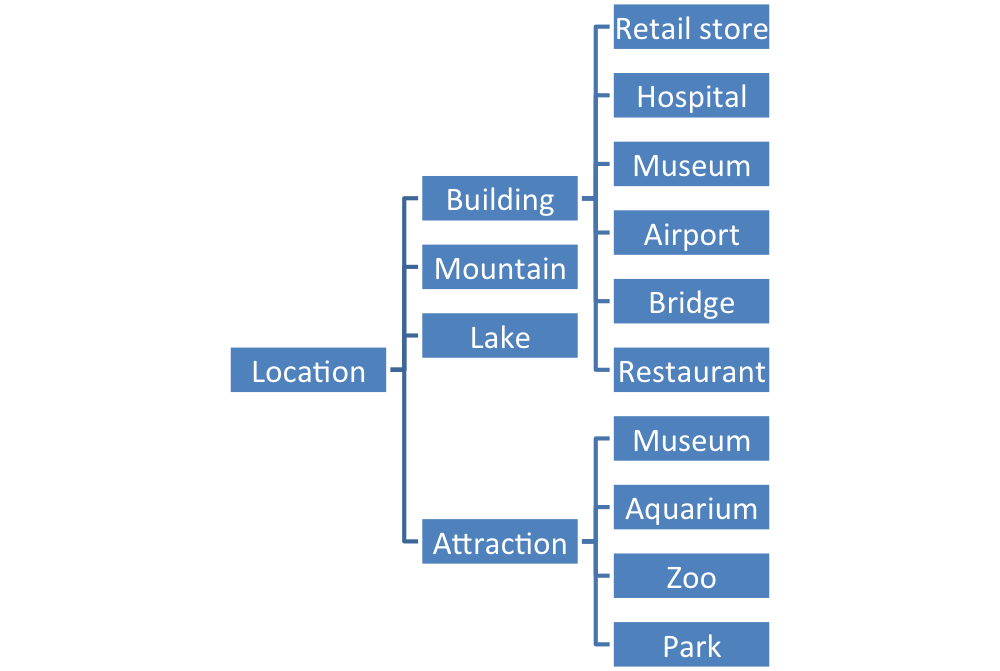
\includegraphics[width=0.85\columnwidth]{fig/exp-ontology}
        \caption{A labeling tree based on the text categorization dataset RCV1, from Mo et al.}
        \label{fig:exp-ontology}
    \end{figure}
\end{frame}
\begin{frame}
    \frametitle{Hierarchical Active Learning}
    \framesubtitle{}
    \begin{figure}[!htb]
        \centering
        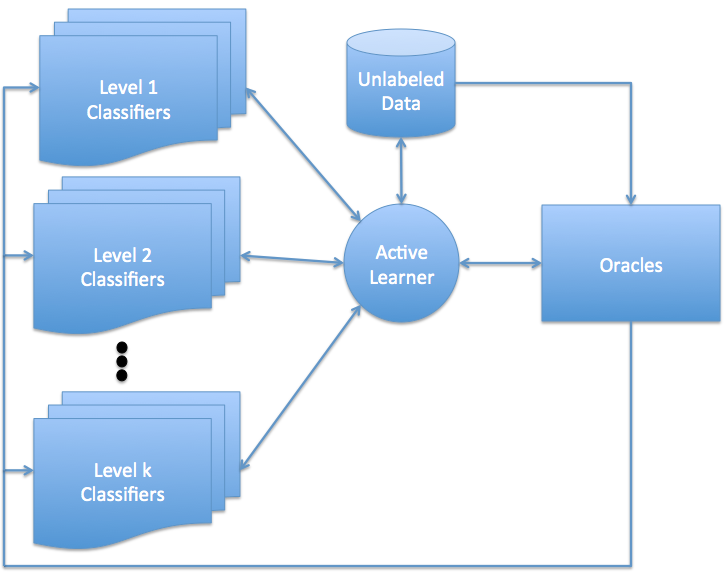
\includegraphics[width=0.65\columnwidth]{fig/AL2}
        \caption{Diagram of HAL approach}
        \label{fig:HALapproach}
    \end{figure}
\end{frame}
\begin{frame}
    \frametitle{Dynamically Adapting Purchase Proportions}
    \framesubtitle{}
    \begin{itemize}
      \item HAL is a fixed-fine ratio methodology.
      \item It takes as input a purchase proportion
vector $p$, which specifies how much of the budget should be used to purchase at
a given level in the hierarchy.
      \item The task of choosing the
level of granularity to purchase labels is framed as a multi-armed bandit problem,
and solved using Auer et al.'s $\epsilon$-greedy bandit algorithm (BANDIT) From Auer et al.
    \end{itemize}
\end{frame}







\section{Related Work}
\begin{frame}
    \frametitle{Related Work}
    \framesubtitle{}
    \begin{itemize}
      \item The experiments and methods described in this work
demonstrate how leveraging fine-grained label  information
can improve the accuracy of a coarse-grained (root-level) classifier, and
 investigate active learning in a hierarchical setting where
 label acquisition cost can vary, from Mo et al.
    \end{itemize}
\end{frame}
\begin{frame}
    \frametitle{Application to Dispatch Dataset}
    \framesubtitle{}
    \par Analysis and evaluation follow Mo et al.'s work.
    \begin{itemize}
      \item Fine outperforms Coarse in PR-AUC
      \item Active outperforms Passive in PR-AUC
      \item HAL ran with variable cost, fine proportions and budget
      \item BANDIT approach shown to be robust to changes in cost and budget
    \end{itemize}
\end{frame}








\section{Exp. Setup}
\begin{frame}
    \frametitle{Training and Testing Coarse-Grain and Fine-Grain Classifiers}
    \framesubtitle{}
\end{frame}







\section{Conv. ML}
\begin{frame}
    \frametitle{SVM and Logit Classifier Performance}
    \framesubtitle{Conventional ML}
    \begin{table}[H]
    \centering
    \caption{Logit entire dataset results after parameter tuning}
    \label{tab:LogRegAll-Wt23}
    \resizebox{0.9\columnwidth}{!}{%
    \begin{tabular}{|l||l||l||l||l||l||l|} \hline
    Title & PR & ROC & Acc & F1 & conf (tn/fn) & conf (fp/tp) \\ \hline
    coarse & 0.870 & 0.871 & 0.787 & 0.268 & ( 1503.2 / 17.8 ) & ( 410.4 / 78.3 ) \\
    fine & 0.875 & 0.871 & 0.913 & 0.403 & ( 1776.5 / 37.3 ) & ( 137.1 / 58.8 ) \\ \hline
    \end{tabular}
    }
    \end{table}
    \begin{table}[H]
    \centering
    \caption{SVM entire dataset results after parameter tuning}
    \label{tab:SVM-All}
    \resizebox{0.9\columnwidth}{!}{%
    \begin{tabular}{|l||l||l||l||l||l||l|}\hline
    Title & PR & ROC & Acc & F1 & conf (tn/fn) & conf (fp/tp) \\ \hline
    coarse & 0.892 & 0.880 & 0.866 & 0.347 & ( 1669.5 / 24.8 ) & ( 244.1 / 71.3 ) \\
    fine & 0.898 & 0.882 & 0.942 & 0.485 & ( 1839.0 / 41.5 ) & ( 74.6 / 54.6 ) \\ \hline
    \end{tabular}
    }
    \end{table}
\end{frame}
\begin{frame}
    \frametitle{SVM and Logit Classifier Performance}
    \framesubtitle{F-measure Analysis}
    \begin{figure}[!htb]
        \centering
        \begin{subfigure}[t]{0.475\textwidth}
            \centering
            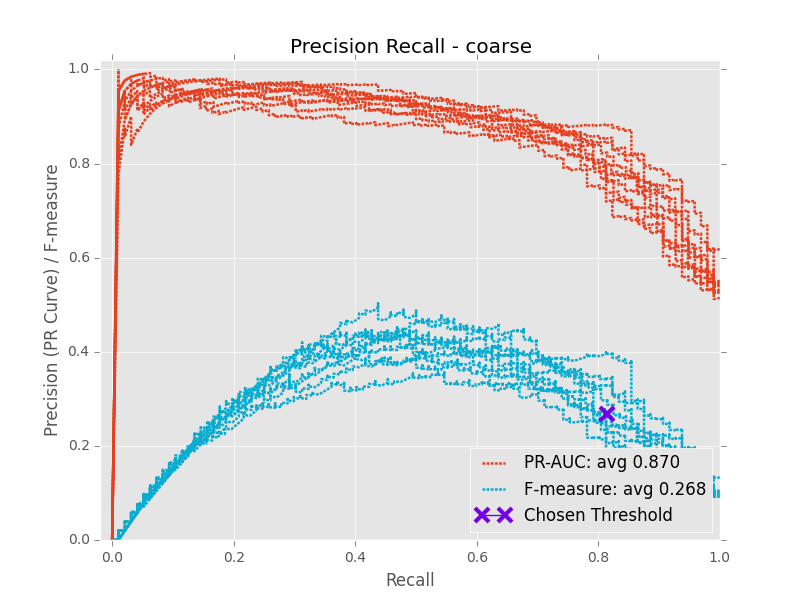
\includegraphics[width=\textwidth]{fig/LogReg_FindThreshold_PrCurve_coarse}
            \caption{Log Reg Pr Curves - Coarse}
        \end{subfigure}
        ~
        \begin{subfigure}[t]{0.475\textwidth}
            \centering
            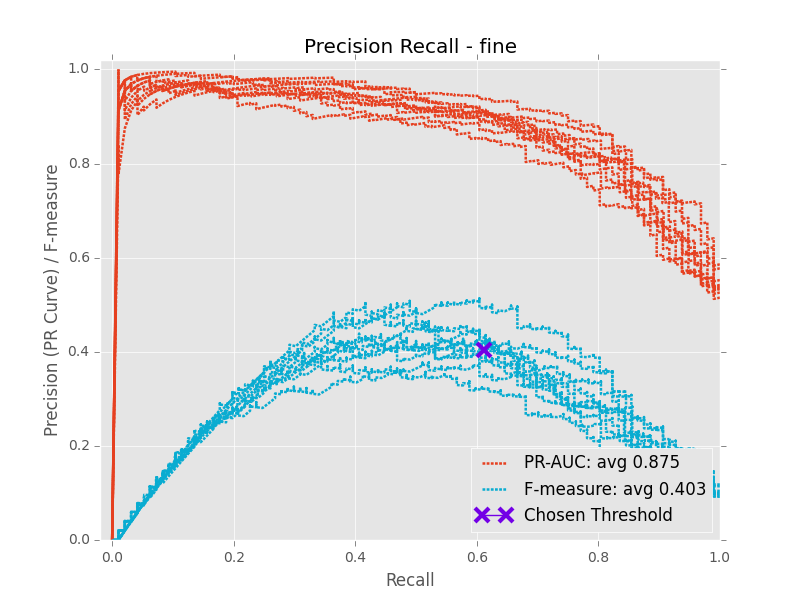
\includegraphics[width=\textwidth]{fig/LogReg_FindThreshold_PrCurve_fine}
            \caption{Log Reg Pr Curves - Fine}
        \end{subfigure}
        \caption{The fine default threshold occurs at a point on the PR curve associated with a higher
        F-measure score compared to the coarse curves.}
        \label{fig:LogRegThreshPr}
    \end{figure}
\end{frame}
\begin{frame}
    \frametitle{SVM and Logit Classifier Performance}
    \framesubtitle{F-measure Analysis}
    \begin{figure}[!htb]
        \centering
        \begin{subfigure}[t]{0.475\textwidth}
            \centering
            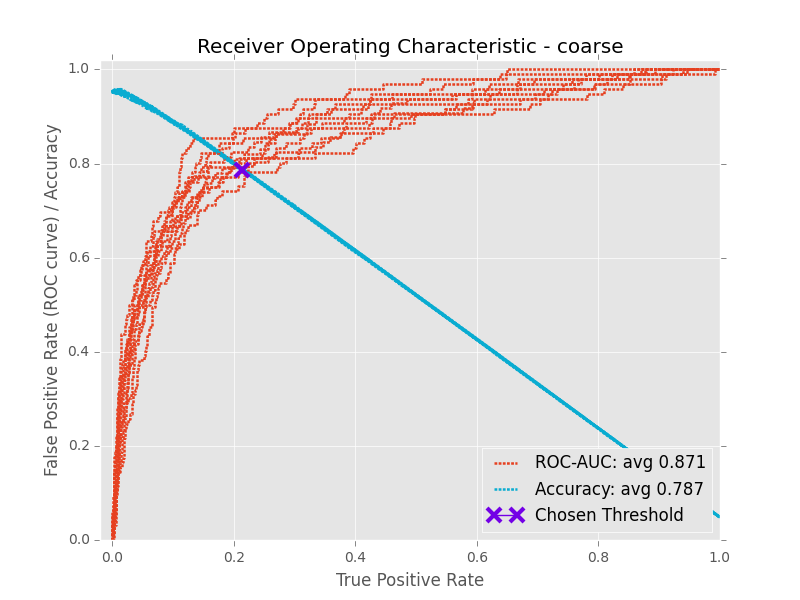
\includegraphics[width=\textwidth]{fig/LogReg_FindThreshold_RocCurve_coarse}
            \caption{Log Reg ROC Curves - coarse}
        \end{subfigure}%
        ~
        \begin{subfigure}[t]{0.475\textwidth}
            \centering
            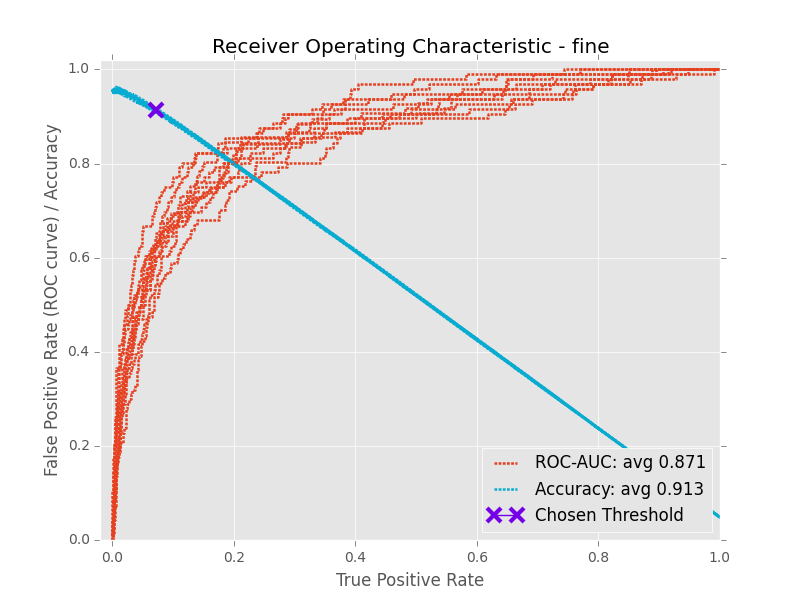
\includegraphics[width=\textwidth]{fig/LogReg_FindThreshold_RocCurve_fine}
            \caption{Log Reg ROC Curves - fine}
        \end{subfigure}
        \caption{Fine has a higher accuracy than coarse at the default threshold for the Logit classifier.}
        \label{fig:LogRegThreshAcc}
    \end{figure}
\end{frame}







\section{Act. vs Pass.}
\begin{frame}
    \frametitle{Active vs. Passive Curve Analysis}
    \framesubtitle{Logit PR-AUC curves}
    \begin{figure}[!htb]
        \centering
        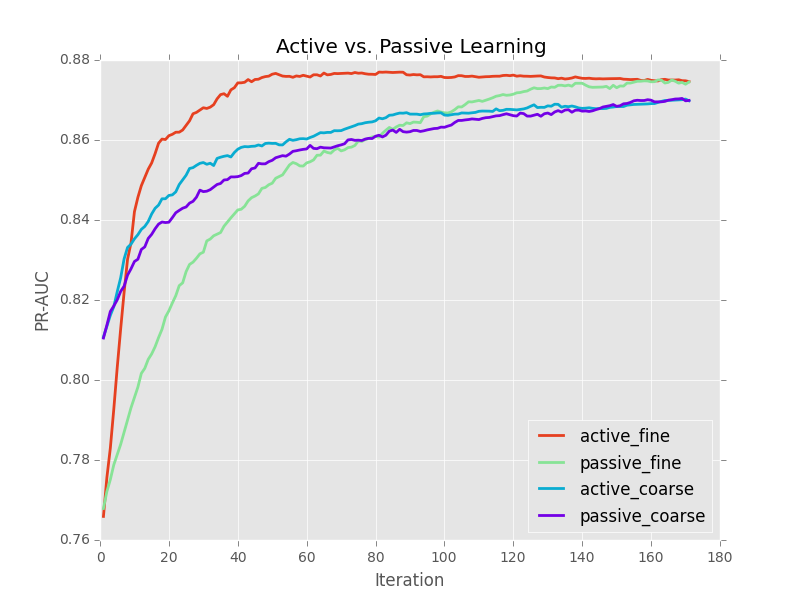
\includegraphics[width=0.70\columnwidth]{fig/runActPassLogReg_pr}
        \caption{The PR-AUC curves for rounds with the Logistic
    Regression classifier conforms to expectations, with active fine having
    the best performance, and Active outperforming Passive for both coarse
    and fine classifier types.}
    \label{fig:runActPassLogReg_pr}
    \end{figure}
\end{frame}
\begin{frame}
    \frametitle{Active vs. Passive Curve Analysis}
    \framesubtitle{Logit ROC-AUC curves}
    \begin{figure}[!htb]
        \centering
        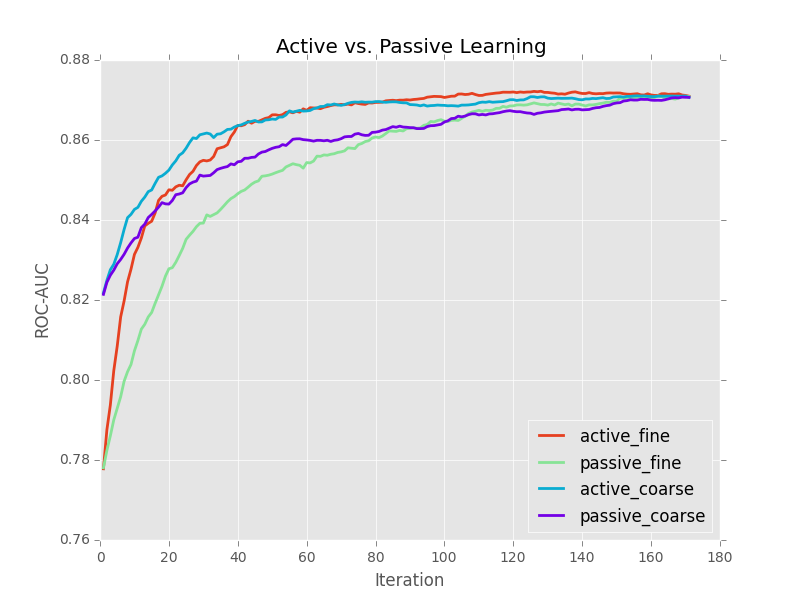
\includegraphics[width=0.70\columnwidth]{fig/runActPassLogReg_roc}
        \caption{The ROC-AUC curves for rounds with the
    Logistic Regression classifier. The active curves beat out the passive
    curves for both coarse and fine.}
%    Note that active fine ROC curve doesn't
%    converge to the active coarse ROC curve until round 40. This is contrasted
%    to a dominance of the active fine PR curve after round 10.}
    \label{fig:runActPassLogReg_roc}
    \end{figure}
\end{frame}
\begin{frame}
    \frametitle{Active vs. Passive Curve Analysis}
    \framesubtitle{Logit Accuracy}
    \begin{figure}[!htb]
        \centering
        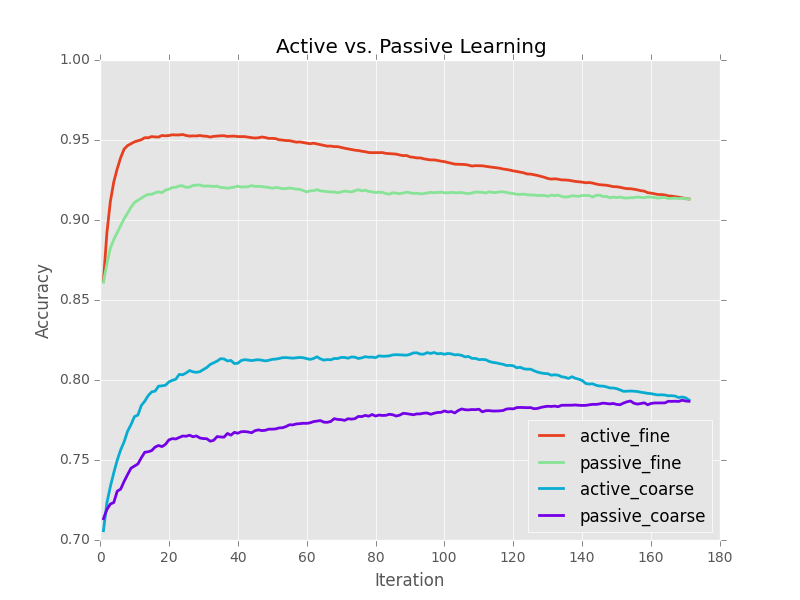
\includegraphics[width=0.70\columnwidth]{fig/runActPassLogReg_acc}
        \label{fig:runActPassLogReg_acc}
        \caption{The accuracy of the classifiers stays at
roughly the same rate throughout the rounds; this is due to an effective
weighting scheme.}
    \end{figure}
\end{frame}
\begin{frame}
    \frametitle{Active vs. Passive Curve Analysis}
    \framesubtitle{Logit F-measure}
    \begin{figure}[!htb]
        \centering
        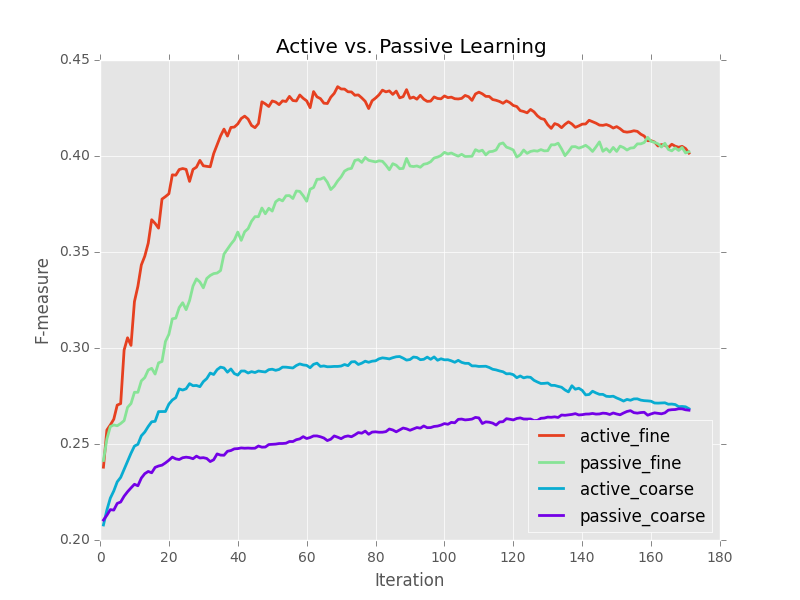
\includegraphics[width=0.70\columnwidth]{fig/runActPassLogReg_f1}
        \label{fig:runActPassLogReg_f1}
        \caption{Both curves show a dominance of fine over coarse and
Active over Passive.}
    \end{figure}
\end{frame}
\begin{frame}
    \frametitle{Active vs. Passive Curve Analysis}
    \framesubtitle{SVM PR-AUC curves}
    \begin{figure}[!htb]
        \centering
        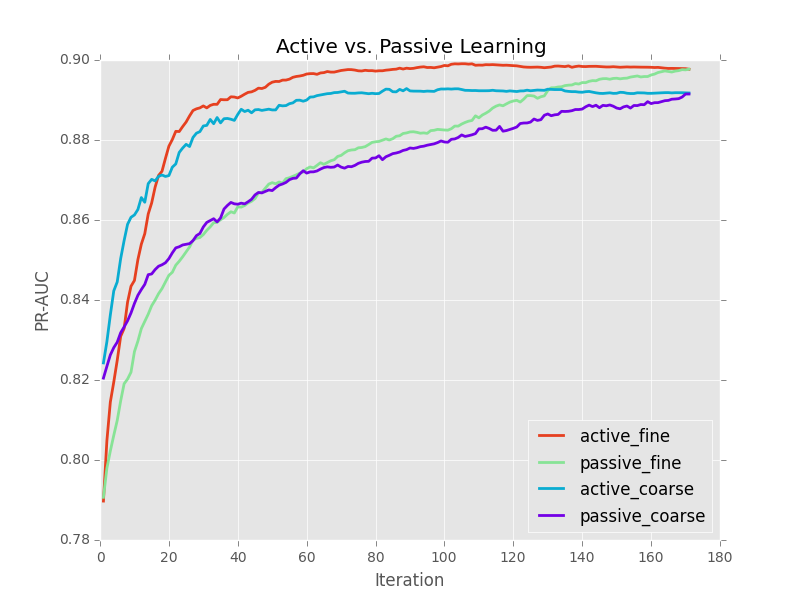
\includegraphics[width=0.70\columnwidth]{fig/runActPassSVM_pr}
        \label{fig:ActiveVsPassivePRSVM}
        \caption{The PR AUC curves for SVM show a slight advantage for active fine,
         similar to the Logit results.}
    \end{figure}
\end{frame}
\begin{frame}
    \frametitle{Active vs. Passive Curve Analysis}
    \framesubtitle{SVM ROC-AUC curves}
    \begin{figure}[!htb]
        \centering
        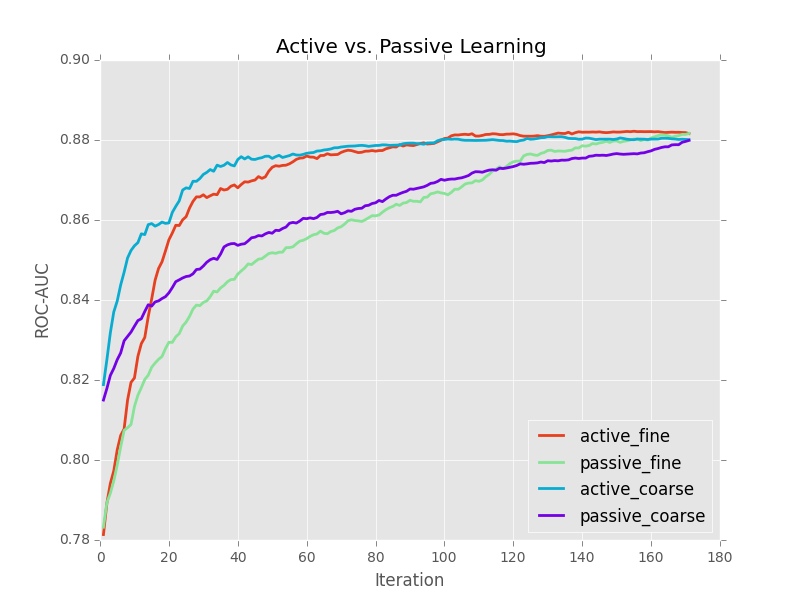
\includegraphics[width=0.70\columnwidth]{fig/runActPassSVM_roc}
        \label{fig:ActiveVsPassiveROCSVM}
        \caption{The ROC AUC curves for SVM match the Logit results, the convergence of
         active fine to active coarse takes slightly longer, round 60 compared to round 40.}
    \end{figure}
\end{frame}








\section{FFR Results}
\begin{frame}
    \frametitle{Plots for Fine Fixed Ratio Results}
    \framesubtitle{Fine Cost 1}
    \begin{figure}[!htb]
	\centering
    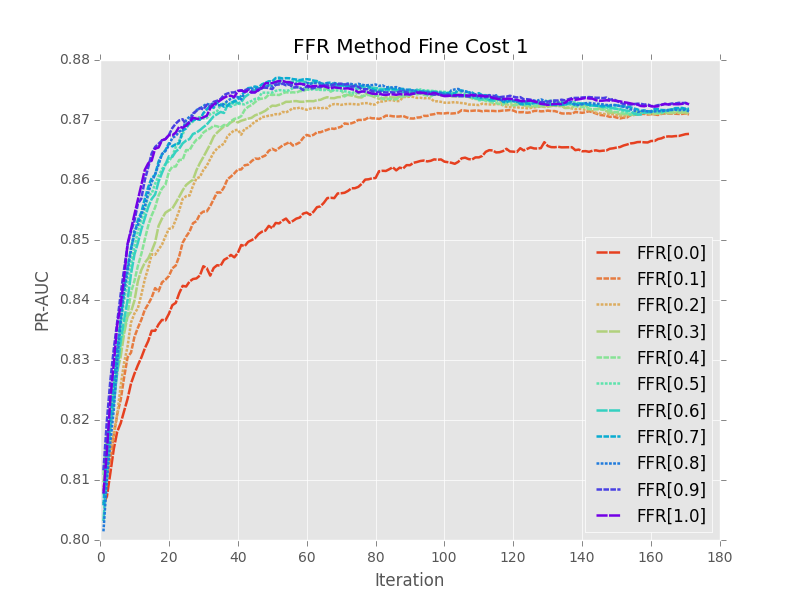
\includegraphics[width=0.7\columnwidth]{fig/ParamsFFR_PR_Cost1_rnds0_180}
    \caption{For this curve the fine and coarse grain labels
    both have a cost of 1.}
%    The purple 1.0 curve shows that if only fine-grained labels
%    are purchased, the highest performing PR-AUC can be obtained. All FFR ratios end at the same round
%    since the cost of the fine and coarse instances is the same the budget.}
%    \label{fig:ParamsFFR_PR_Cost1_rnds0_180}
\end{figure}
\end{frame}
\begin{frame}
    \frametitle{Plots for Fine Fixed Ratio Results}
    \framesubtitle{Fine Cost 2}
    \begin{figure}[!htb]
        \centering
        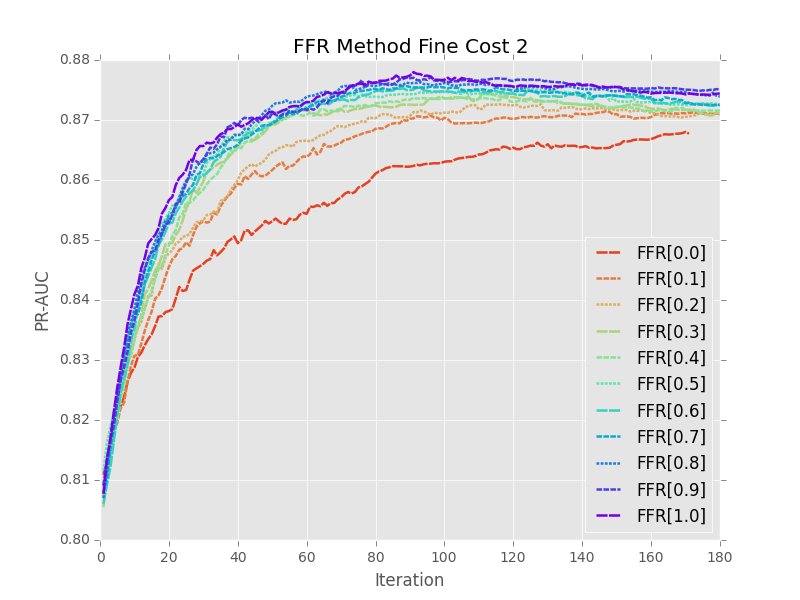
\includegraphics[width=0.7\columnwidth]{fig/ParamsFFR_PR_Cost2_rnds0_180}
        \caption{At fine cost 2, advantage of the higher FFR values decreases but the ordering
        of the curves remains unchanged.}
        \label{fig:ParamsFFR_PR_Cost2_rnds0_180}
    \end{figure}
\end{frame}
\begin{frame}
    \frametitle{Plots for Fine Fixed Ratio Results}
    \framesubtitle{Fine Cost 4}
    \begin{figure}[!htb]
        \centering
        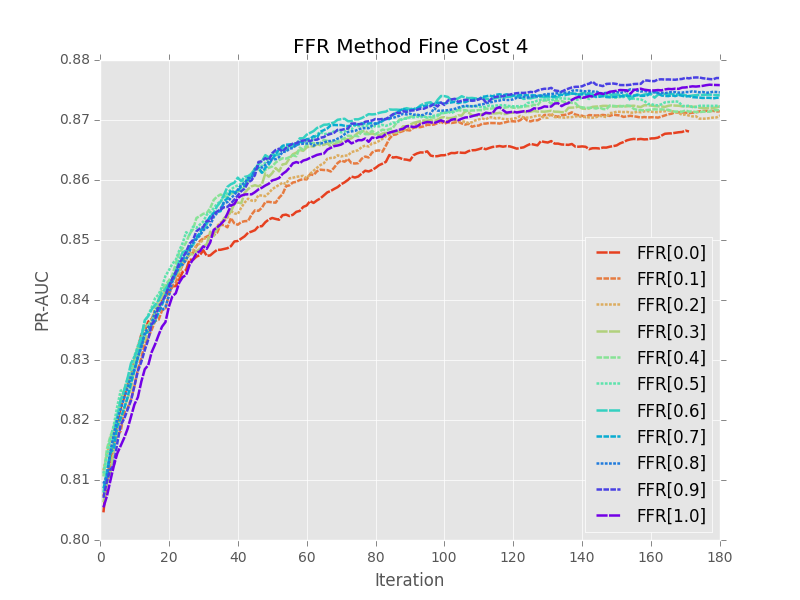
\includegraphics[width=0.7\columnwidth]{fig/ParamsFFR_PR_Cost4_rnds0_180}
        \caption{At fine cost 4, the highest FFR $1.0$ is no longer preferred, the
        cost is to high for fine instances PR-AUC utility to overcome the PR-AUC
        increase gained by purchasing more coarse instances.}
        \label{fig:ParamsFFR_PR_Cost4_rnds0_180}
    \end{figure}
\end{frame}
\begin{frame}
    \frametitle{Plots for Fine Fixed Ratio Results}
    \framesubtitle{Fine Cost 8}
    \begin{figure}[!htb]
        \centering
        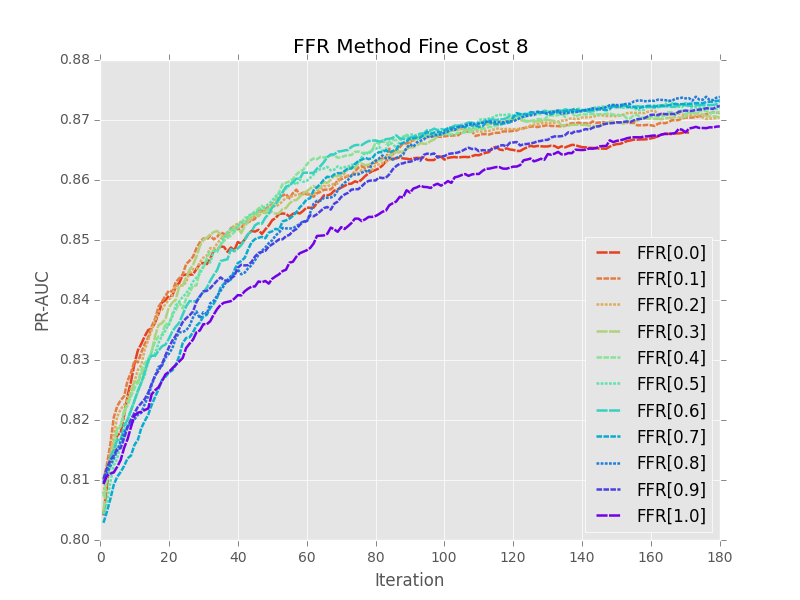
\includegraphics[width=0.7\columnwidth]{fig/ParamsFFR_PR_Cost8_rnds0_180}
        \caption{At fine cost 8 the middle FFR values outperform the extreme values
        for rounds 0 to 180.}
        \label{fig:ParamsFFR_PR_Cost8_rnds0_180}
    \end{figure}
\end{frame}
\begin{frame}
    \frametitle{Plots for Fine Fixed Ratio Results}
    \framesubtitle{Fine Cost 8 - Rnds to 500}
    \begin{figure}[!htb]
        \centering
        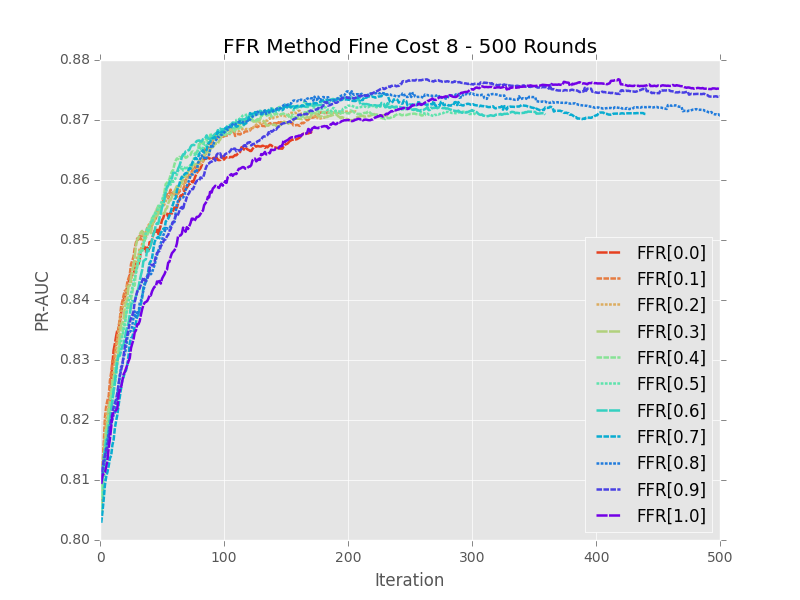
\includegraphics[width=0.7\columnwidth]{fig/ParamsFFR_PR_Cost8_rnds0_500}
        \caption{This shows the iterations continuing through round 500, the curves
        with the higher fine rates eventually settle to the same end point that the
        curves with the high rates of coarse labels purchased achieved at previous
        iterations.}
        \label{fig:ParamsFFR_PR_Cost8_rnds0_500}
    \end{figure}
\end{frame}
\begin{frame}
    \frametitle{Plots for Fine Fixed Ratio Results}
    \framesubtitle{Fine Cost 8 - Rnds 20 to 60}
    \begin{figure}[!htb]
        \centering
        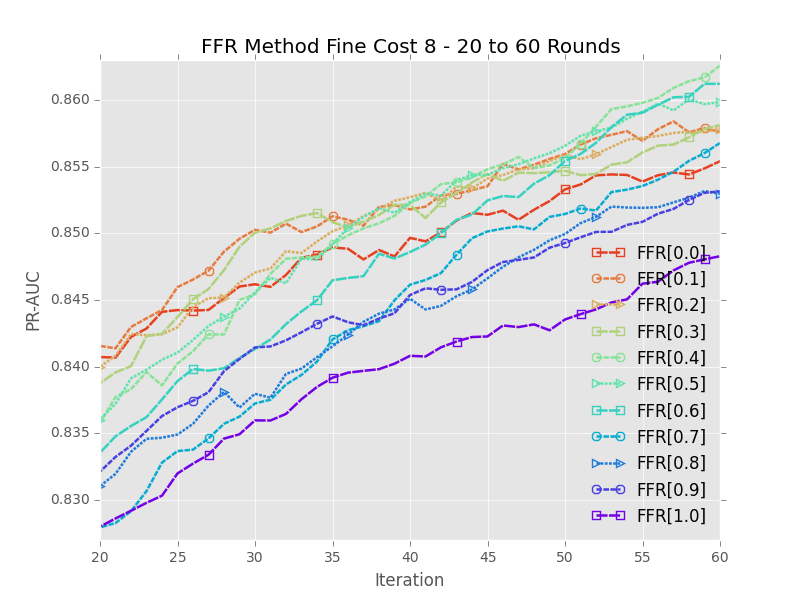
\includegraphics[width=0.7\columnwidth]{fig/ParamsFFR_PR_Cost8_rnds20_60}
        \caption{The fine cost 8 curves shown expanding the rounds 20-60. If a round budget of 40
        occurs than the recommended FFR would be $0.2$.}
        \label{fig:ParamsFFR_PR_Cost8_rnds20_60}
    \end{figure}
\end{frame}
\begin{frame}
    \frametitle{Plots for Fine Fixed Ratio Results}
    \framesubtitle{Fine Cost 16}
    \begin{figure}[!htb]
        \centering
        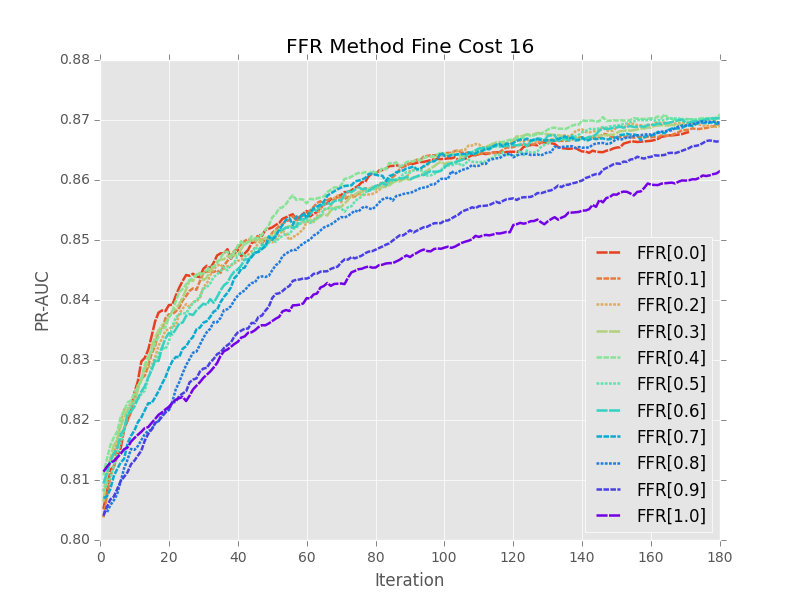
\includegraphics[width=0.7\columnwidth]{fig/ParamsFFR_PR_Cost16_rnds0_180}
        \caption{The fine cost is increased to 16. The cost is to high for the fine label advantage to offset
        the decreased number of instances purchased.}
        \label{fig:ParamsFFR_PR_Cost16_rnds0_180}
    \end{figure}
\end{frame}









\section{BANDIT Res.}
\begin{frame}
    \frametitle{BANDIT Approach Results}
    \framesubtitle{Varying Cost Analysis - Plot}
    \begin{figure}[!htb]
        \centering
        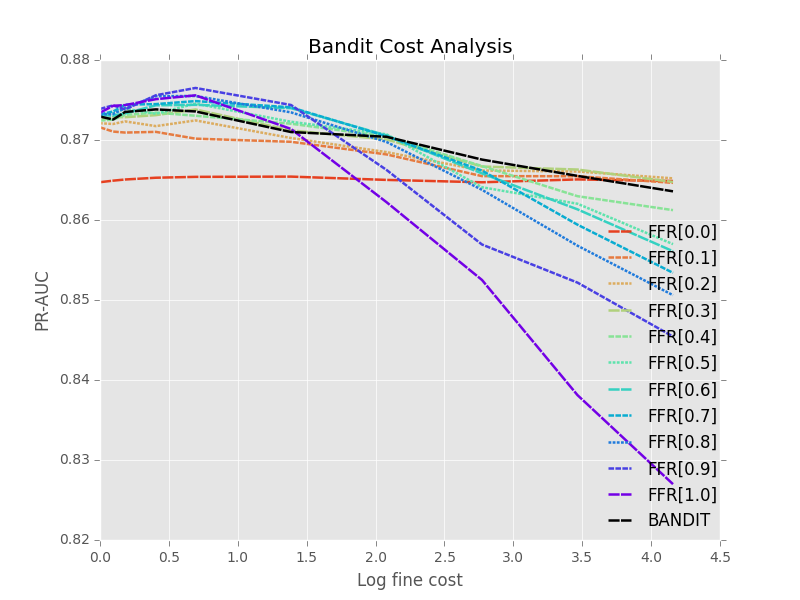
\includegraphics[width=0.70\columnwidth]{fig/BanditPlotLogFine}
        \caption{BANDIT log fine cost analysis with budget fixed.}
        \label{fig:BanditPlotLogFine}
    \end{figure}
\end{frame}
\begin{frame}
    \frametitle{BANDIT Approach Results}
    \framesubtitle{Varying Cost Analysis - Rank and Diff Metrics}
        \begin{table}[H]
        \caption{Aggregated PR AUC for the protein dataset}
        \centering
        \resizebox{0.9\columnwidth}{!}{%
        \begin{tabular}{lrrrrrrrr}
        \hline
        {} &  diff &       &       &       & rank &     &        &       \\
        {} &   min &   max &  mean &   std &  min & max &   mean &   std \\
        \hline
        algorithm &       &       &       &       &      &     &        &       \\
        BANDIT & 0.000 & 0.003 & \underline{\textbf{0.001}} & 0.001 & 0 & 8 & 4.8 & 2.315 \\
        FFR[$0.0$] & 0.000 & 0.011 & 0.007 & 0.004 & 1 & 11 & 8.8 & 3.429 \\
        FFR[$0.1$] & 0.001 & 0.006 & 0.003 & 0.002 & 3 & 10 & 8.0 & 2.793 \\
        FFR[$0.2$] & 0.000 & 0.004 & 0.002 & 0.001 & 0 & 9 & 6.5 & 3.500 \\
        FFR[$0.3$] & 0.000 & 0.003 & 0.001 & 0.001 & 0 & 8 & 5.1 & 2.663 \\
        FFR[$0.4$] & 0.000 & 0.004 & 0.002 & 0.001 & 1 & 8 & 5.6 & 2.200 \\
        FFR[$0.5$] & 0.000 & 0.008 & 0.002 & 0.002 & 0 & 8 & 4.6 & 2.200 \\
        FFR[$0.6$] & 0.000 & 0.009 & 0.002 & 0.003 & 1 & 7 & 4.6 & 1.855 \\
        FFR[$0.7$] & 0.000 & 0.012 & 0.002 & 0.004 & 0 & 8 & \underline{\textbf{3.3}} & 2.571 \\
        FFR[$0.8$] & 0.000 & 0.015 & 0.003 & 0.005 & 1 & 9 & 4.8 & 3.027 \\
        FFR[$0.9$] & 0.000 & 0.020 & 0.005 & 0.007 & 0 & 10 & 4.3 & 4.605 \\
        FFR[$1.0$] & 0.000 & 0.038 & 0.009 & 0.013 & 1 & 11 & 5.6 & 4.630 \\
        \hline
        \end{tabular}}
        \label{tab:banditLogFine}
        \end{table}
\end{frame}
\begin{frame}
    \frametitle{BANDIT Approach Results}
    \framesubtitle{Varying Budget Analysis - Mixed Cost}
    \begin{figure}[!htb]
        \centering
        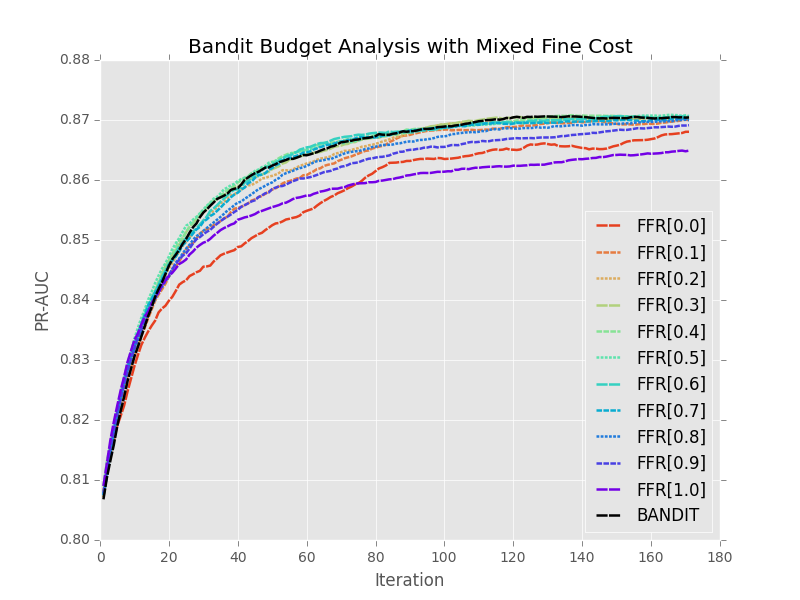
\includegraphics[width=0.70\columnwidth]{fig/BanditMixedCostPR}
        \caption{BANDIT mixed fine cost plot.}
        \label{fig:BanditMixedCostPR}
    \end{figure}
\end{frame}
\begin{frame}
    \frametitle{BANDIT Approach Results}
    \framesubtitle{BANDIT - Rnds 20 to 60}
    \begin{figure}[!htb]
        \centering
        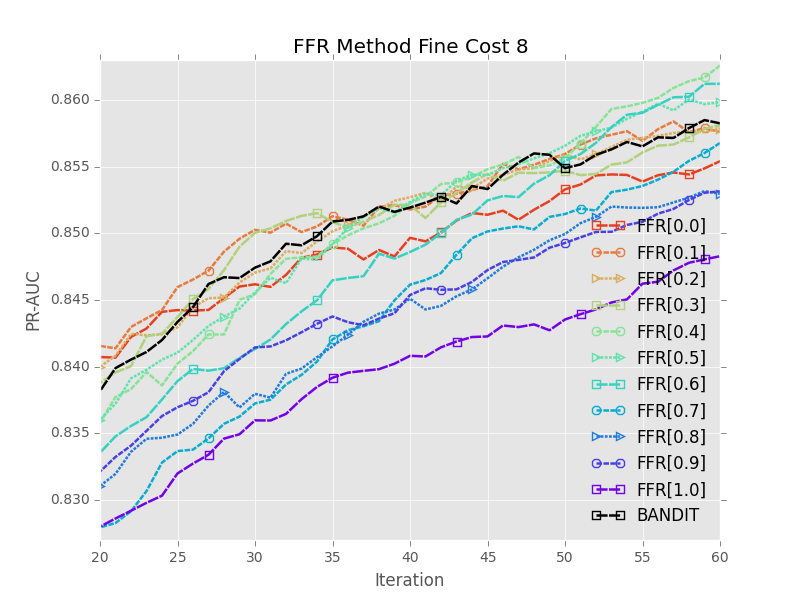
\includegraphics[width=0.70\columnwidth]{fig/BANDIT_PR_Cost8_rnds20_60}
        \caption{
        The fine cost 8 curves shown expanding the rounds 20-60. With the BANDIT approach
        plotted. At budget iteration 40, BANDIT PR-AUC is within $0.0007$ of the top learner's
        PR-AUC.
        }
        \label{fig:BANDIT_PR_Cost8_rnds20_60}
    \end{figure}
\end{frame}







\section{Conclusions}
\begin{frame}
    \frametitle{Conclusions and Future Work}
    \framesubtitle{}
\end{frame}














%\begin{frame}
%    \frametitle{Introduction}
%    \framesubtitle{}
%    \texttt{Beamer} is a wonderful \LaTeX\ document class that produces
%    high quality PDF slide presentations.
%    Moreover, you can customize and develop your own themes!
%\end{frame}


%\section{UNL Theme}
%\begin{frame}
%    \frametitle{UNL Theme}
%    \framesubtitle{}
%    This theme was developed for the University of Nebraska--Lincoln.
%    The theme itself was developed from the PaloAlto, sidebar and sidbartab
%    themes available by default in beamer.
%    However, this theme has several unique features and customizations:
%    \begin{itemize}
%      \item The color theme uses UNL's ``scarlet and creme'' colors.
%      \item Improved spacing.
%      \item Math mode preserves \LaTeX's serif font.
%      \item Incorporates UNL's Logo automatically.
%      \item Unique drop shadows on the top and side bars!
%    \end{itemize}
%\end{frame}
%
%
%\begin{frame}
%    \frametitle{Other Features}
%    \framesubtitle{}
%    For convenience, if you are in handout mode, all features, including the
%    navigation symbols at the bottom right are shut off!
%    Beamer boxes are by default, rounded and have a drop shadow.  All beamer
%    boxes (definition, theorem, etc) have the same color scheme.
%    \begin{definition}
%      This is my definition
%      $$A = \{p \mid \textrm{$p$ is prime }\}$$
%    \end{definition}
%    \begin{theorem}
%      The set $A$ is countable.
%    \end{theorem}
%\end{frame}
%
%

%\section{Using The Theme}
%\begin{frame}[fragile]
%    \frametitle{How To Use The Theme}
%    \framesubtitle{Theme Options}
%    To use the UNL Theme, after your document class declaration, simply use:
%    \begin{verbatim}\usetheme{UNLTheme}\end{verbatim}
%    To pass options to the package, use
%    \verb"\usetheme[left,hideothersubsections,width=2.5cm]{UNLTheme}"
%\end{frame}
%
%\begin{frame}[fragile]
%    \frametitle{How To Use The Theme}
%    \framesubtitle{Theme Options}
%    There are also several options that you can pass:
%    \begin{itemize}
%      \item \texttt{hideothersubsections} -- This hides subsections in the
%            sidebar \emph{other than} the subsections of the current section.
%      \item \texttt{hideallsubsections} -- This option doesn't print \emph{any}
%            subsections in the sidebar.
%      \item \texttt{width} -- sets the width of the sidebar, default is
%      	    \verb"2.5\baselineskip"
%      \item \texttt{height} -- sets the height of the header, default is
%      	    \verb"2.5\baselineskip"
%      \item \texttt{left} -- sets the sidebar to the left of the slide (default).
%      \item \texttt{right} -- sets the sidebar to the right of the slide.
%    \end{itemize}
%\end{frame}
%
%\begin{frame}
%    \frametitle{How To Get The Theme}
%    \framesubtitle{}
%    The theme is available from my home page,
%    \textcolor{blue}{\url{http://www.cse.unl.edu/~cbourke/}}
%    You need \texttt{You need beamerthemeUNLTheme.sty} and \texttt{UNL.pdf}
%    (the UNL logo).
%    Place them in the working directory or add them to \texttt{beamer/themes/theme}
%    or somewhere in your \LaTeX\ path and you're good to go!
%\end{frame}
    
\end{document}
